\section{Visual Studio Code 2023}
Visual Studio ist eine Entwicklerumgebung von Microsoft. Die aktuellste Version ist Visual Studio 2023.
Der einfache aber leistungsstarke Quellcode-Editor, ist für Windows, macOS und Linux verfügbar ist. Er bietet außerdem integrierte Unterstützung für 
JavaScript, TypeScript und Node.js und verfügt über ein umfangreiches Ökosystem von Erweiterungen für andere Sprachen und 
Laufzeiten (z. B. C++, C\#, Java, Python, PHP, Go, .NET).
Visual Studio bietet Syntaxhervorhebung, Code-Vervollständigung, Debugging und viele weitere nützliche Features, die beim 
Coden unterstützen können. \cite{APCW2007}

\subsection*{Bezug auf das Projekt}
Für die Entwicklung des Frontends in React wurde Visual Studio Code verwendet. Der Editor ist kostenlos verfügbar, leichtgewichtig
und schnell. Er lässt sich schnell öffnen und verfügt über eine gute integrierte Git-Unterstützung. Es lassen sich viele 
Erweiterungen oder Extensions installieren für die React-Syntax-Hervorhebung, IntelliSense, Debugging und vieles mehr,
die das Arbeiten in React enorm verbessern können.

\begin{figure}[ht!]
  \centering
  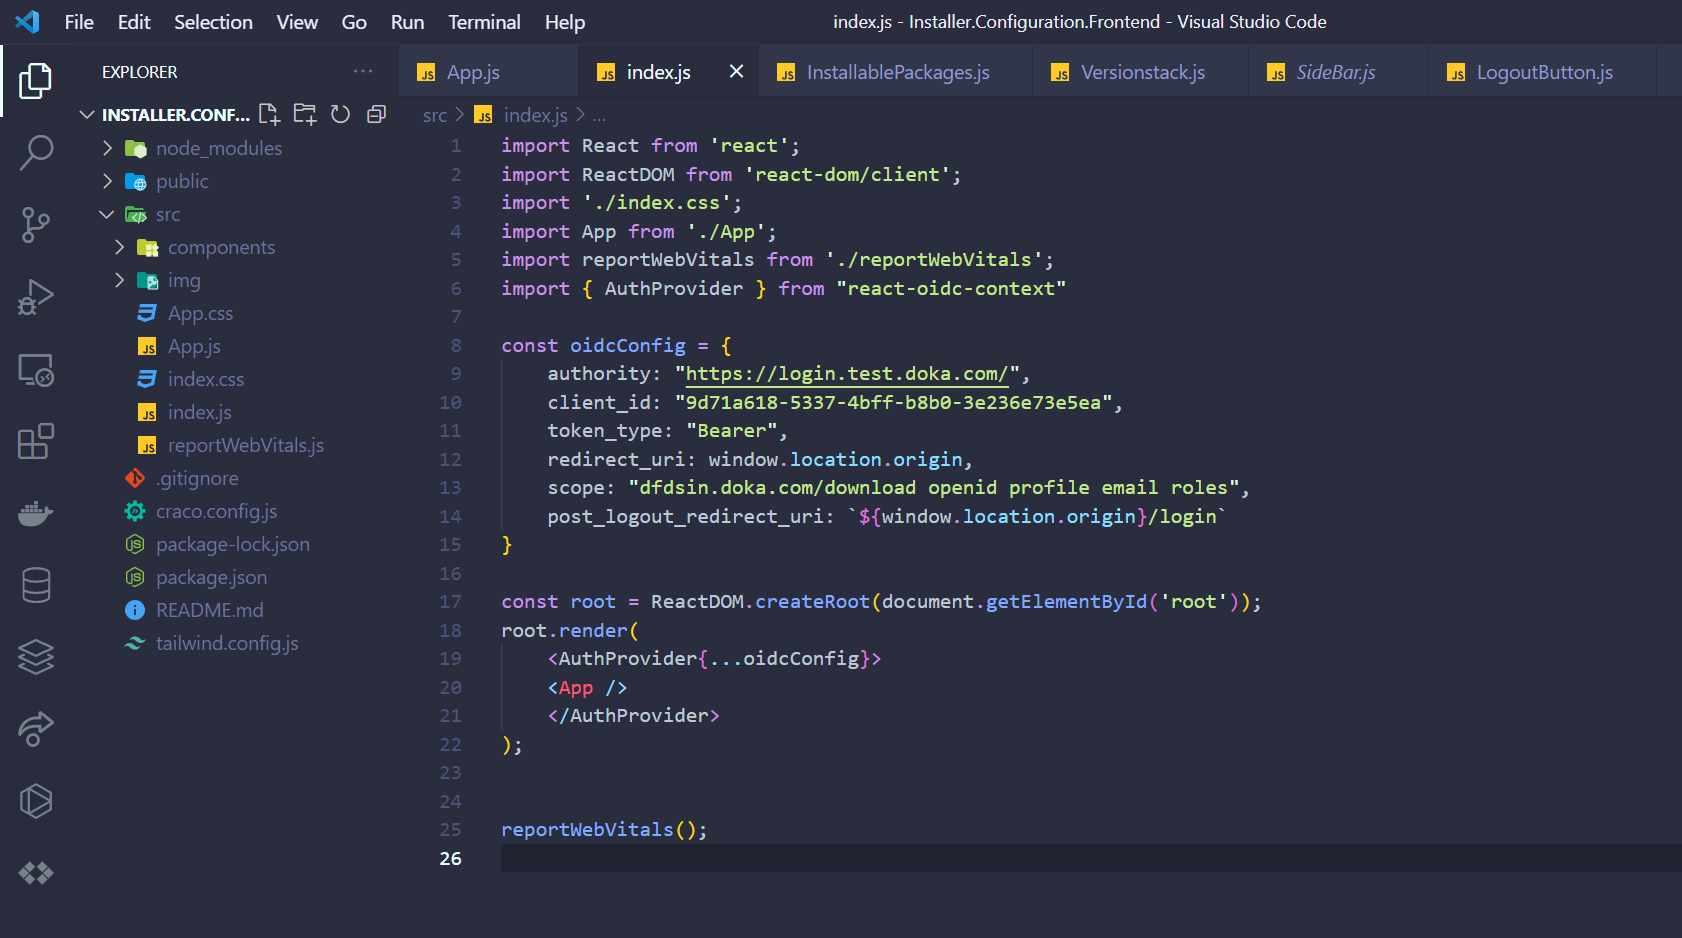
\includegraphics[scale=.4]{pics/visual-studio-code.PNG}
  \caption{\label{fig:The-caption}Visual Studio Code}
  \label{fig:impl:use-case-diagramm}
\end{figure}

\section{Latex}
Normalerweise reichen Textverarbeitungsprogramme wie Word für das Erstellen
von Texten aus. Oft aber reicht das nicht für professionelle Texte, wie zum Beispiel
für Diplomarbeiten, wo die Ansprüche höher sind. LaTeX erfüllt diese Ansprüche eines 
Textverarbeitungsprogramms, jedoch zum Preis der Komplexität. Für Neueinsteiger, die davor nur mit
Word, LibreOffice und ähnliche gearbeitet haben, ist es anfangs etwas gewöhnungsbedürftig.
\\
Latex kümmert sich um die Typografie, um das Layout und andere Gestaltungsmöglichkeiten,
die man zu Beginn festlegen bzw. anpassen kann. Die Idee dahinter ist, dass sich der Autor 
hauptsächlich auf den Inhalt des Textes konzentrieren kann und sich nicht ständig Gedanken um 
das Aussehen machen muss. \cite{APCW2008}


\begin{figure}[ht!]
  \centering
  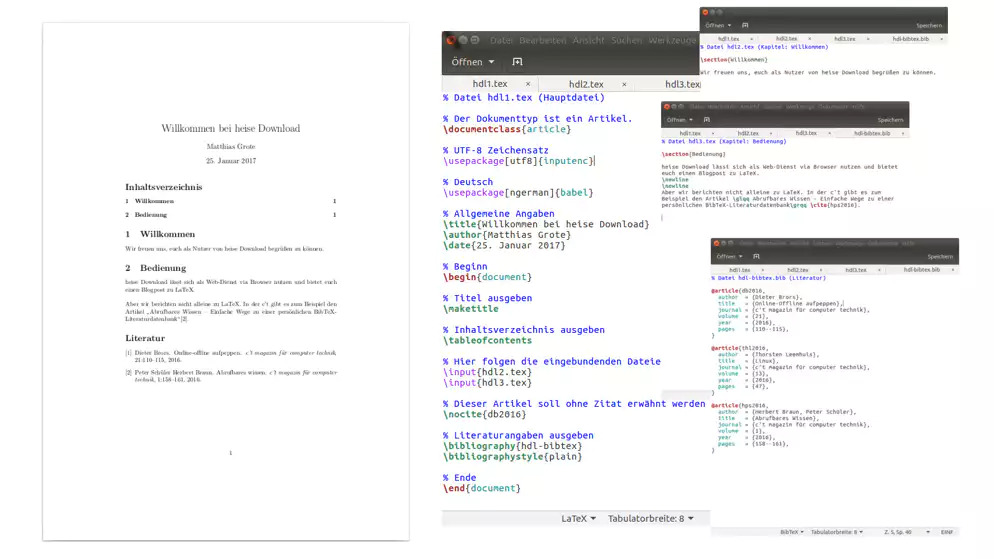
\includegraphics[scale=.4]{pics/latex.jpg}
  \caption{\label{fig:The-caption}Latex \cite{APCW2008}}
  \label{fig:impl:use-case-diagramm}
\end{figure}

Das Textsatzsystem wurde in Kombinatin mit Visual Studio Code verwendet, um diese Arbeit zu schreiben.
Hilfreich dabei war die Visual Studio Erweiterung ``LaTex Workshop'', die grundlegende Funktionen und Hilfen inklusive einer 
Dokumentation, für das arbeiten an LaTex-Dokumenten, bereitstellt.

\begin{figure}[ht!]
  \centering
  
\includegraphics[scale=.7]{pics/latex-workshop.PNG}
  \caption{\label{fig:The-caption}Latex-Workshop}
  \label{fig:impl:use-case-diagramm}
\end{figure}

Die Erweiterung bietet auch eine Strukturübersicht und hilft beim Entfernen von überflüssigen Files und mehr im ``Commands'' Abschnitt.

\begin{figure}[ht!]
  \centering
  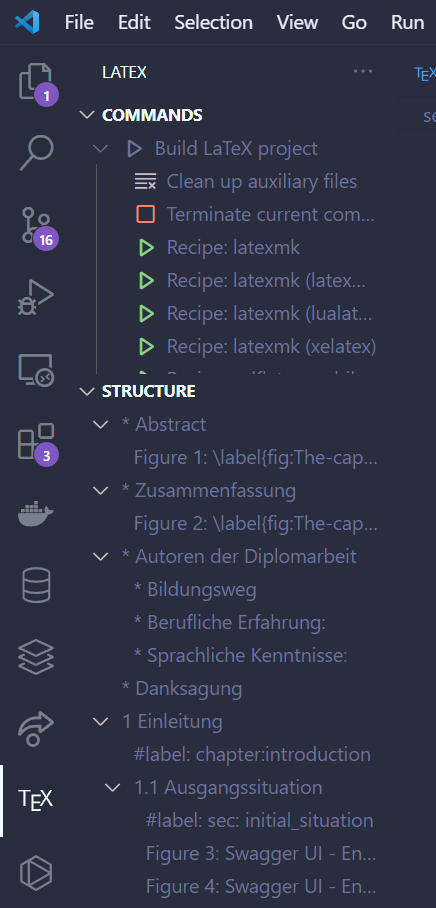
\includegraphics[scale=.8]{pics/latex-workshop-vs-code.PNG}
  \caption{\label{fig:The-caption}Latex-Workshop in VS-Code }
  \label{fig:impl:use-case-diagramm}
\end{figure}

\clearpage

\section{HTML} \label{HTML}
Die Hypertext Markup Language (HTML) strukturiert textbasierte Inhalte 
eines Webdokuments. Neben den Inhalten sind auch Meta-Informationen aufzufinden
die diese Inhalte beschreiben. 

HTML ist einfach zu editieren und kann mit einem beliebigen Texteditor geschrieben werden, 
da es keine speziellen Anforderungen bei der Erstellung gibt. Oft zu finden im HTML Code
sind Tags, die Elemente definieren. Dadurch wird eine Hierarchische Struktur erreicht.
Eine HTML-Seite ist meistens zweigeteilt durch den Head-Tag und den Body-Tag.
\\

\begin{lstlisting}[language=html, caption=HTML Beispiel]
  <html>
  <head>
      <title>My New HTML Page</title>
  </head>
  <body>
    <p>Hello World</p>
  </body>
  </html>
\end{lstlisting}

\subsection*{Head}
Dort werden die Meta-Informationen der Seite festgelegt, die nicht im Browser 
angezeigt werden. Oft werden auch Meta-Tags untergebracht, die für Suchmaschinen 
relevant sein können. 
\subsection*{Body}
Hier befinden sich die eigentlichen Inhalte, die durch den Browser 
visuell dargestellt werden. Beispiele dafür sind, CSS, Mediainhalte, 
Texthervorhebungen und Überschriften. 
\newpage

\section{CSS}
Während HTML für die Strukturierung und den Inhalt der Website zuständigt ist,
sorgen Cascading Stylesheets (CSS) für das Aussehen. Dazu zählen Schriftart, Farbe und
Layout. 
CSS Regeln können mit einem style-Tag im head der HTML Datei festgelegt werden oder
in einer externen CSS-Datei. Diese Datei muss mit einem link-Tag in die Seite eingebunden
werden. 
\\
\begin{lstlisting}[language=html, caption=HTML Beispiel mit CSS]
  <head>
  <link rel="stylesheet" href="style.css">

  <style>
     body { font-family: Helvetica; }
  </style>
<head>
\end{lstlisting}

Man kann CSS aber auch mit dem style-Attribut direkt in den HTML-Tags verwenden.
\begin{lstlisting}[language=html, caption=HTML Beispiel mit CSS]
  <body style="font-family: Helvetica;">
\end{lstlisting}

\subsection*{Aufbau}
Eine CSS-Regel besteht aus zwei Teilen 
\begin{itemize}
  \item {\textbf{CSS-Selektor}, also die Bezeichnung für das angesprochene Element (z.B. h1-Tags, div-Tags,...). }
  \item {\textbf{Eigenschaft und Wert} wie color und green, die dem Element zugewiesen wird.  }
\end{itemize}
Die Kombination aus Eigenschaft : Wert steht in geschweiften Klammern und wird durch
Semikolons getrennt. 
\newpage

\section{Tailwind CSS} \label{TailwindCSS}
Tailwind CSS ist CSS-Framework, welches vorgefertigte CSS-Klassen bereitstellt, die verwendet 
werden können, um HTML-Elemente schnell und einfach zu gestalten. Im Vergleich mit anderen CSS-Frameworks, 
die vorgefertigte UI-Komponenten bereitstellen, fokussiert sich Tailwind mehr auf Low-Level-Bausteine wie 
Abstände (Paddings und Margins), Schriftarten und Farbe, um benutzerdefinierte Styles zu erstellen.

Entwickler können vorgefertigte CSS-Klassen hinzufügen, anstatt für jedes Element benutzerdefiniertes CSS zu 
schreiben \ref{fig:Tailwind}. Das beschleunigt nicht nur den Entwicklungsprozess, sondern kann sich auch positiv auf die Performance 
auswirken. Die Dokumentation von Tailwind CSS ist umfangreich und die große Community erleichtert den Einstieg und 
bietet Unterstützung.\cite{APCW20016}

\begin{figure}[ht!]
    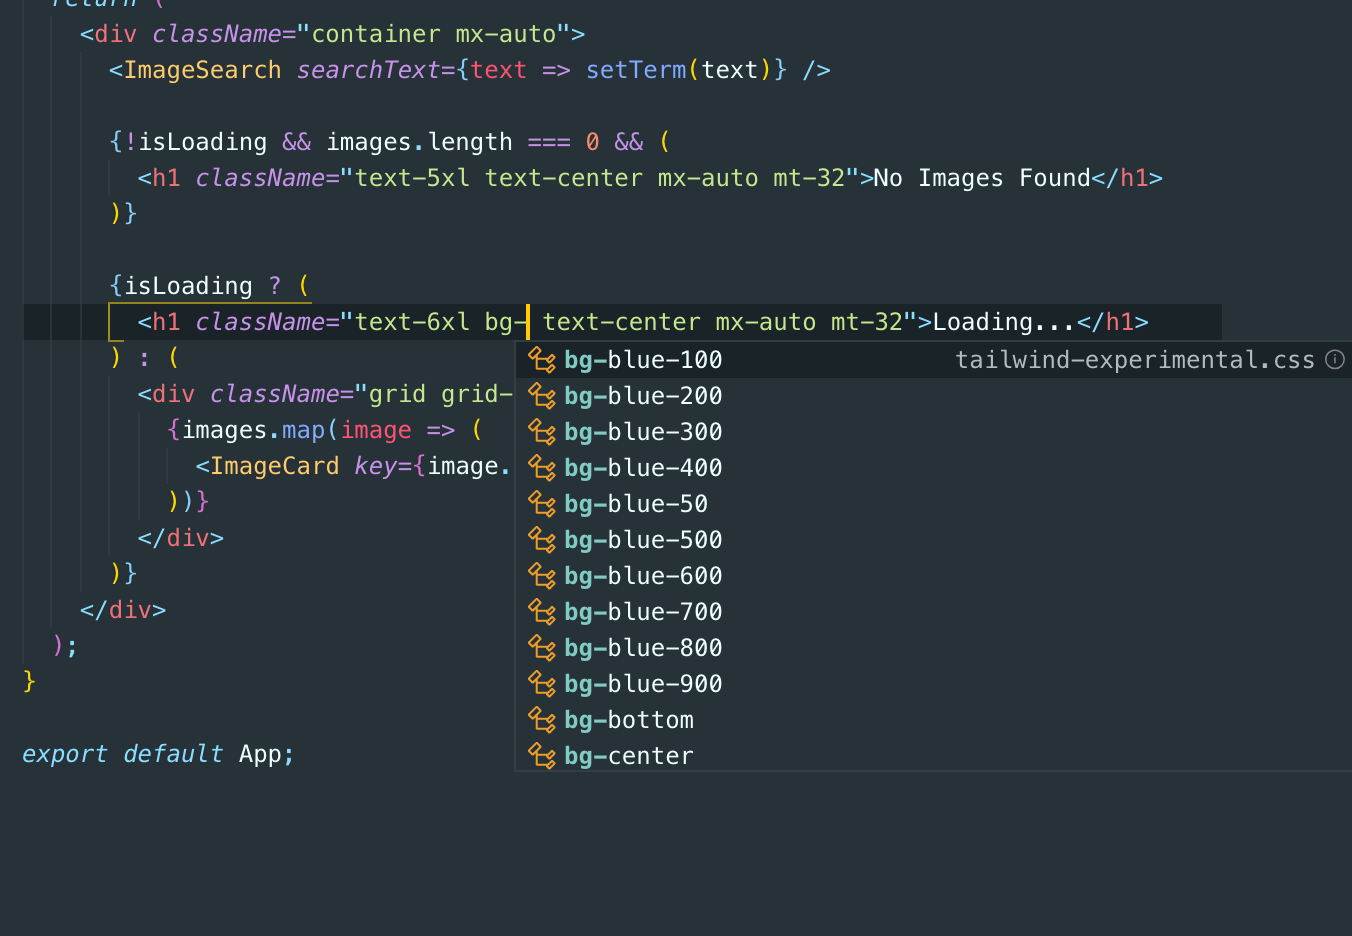
\includegraphics[width=.94\textwidth]{pics/tailwindCSS-class-showcase.png}
    \caption{\label{fig:Tailwind}Tailwind - vorgefertigte CSS-Klassen \cite{APCW20017}}
  \end{figure}

\subsection*{Implementierung}
Vorraussetzungen für die Implementierungen sind ein bestehendes Projekt 
mit einer package.json Datei im Grundverzeichnis. Deswegen sollte natürlich auch Node.js 
auf dem Rechner installiert sein. 
\newpage

Mit folgendem Befehl wird die neueste stabile 
Version von Tailwind CSS als Abhängigkeit installiert. 
\begin{figure}[ht!]
  \centering
  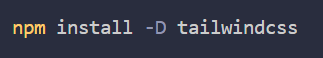
\includegraphics[scale=1.2]{pics/install-tailwind.PNG}
  \caption{\label{fig:Tailwind}TailwindCSS-Framework installieren }
\end{figure}

Als nächstes generiert man die Datei tailwind.config.js mit dem Befehl
\begin{figure}[ht!]
  \centering
  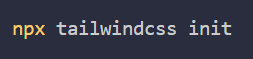
\includegraphics[scale=1.2]{pics/create-tailwind-config.PNG}
  \caption{\label{fig:Tailwind}Tailwind - config-Datei generieren }
\end{figure}

Der Inhalt der Datei sieht ohne eigenes Bearbeiten und Hinzufügen so aus. 
\begin{figure}[ht!]
  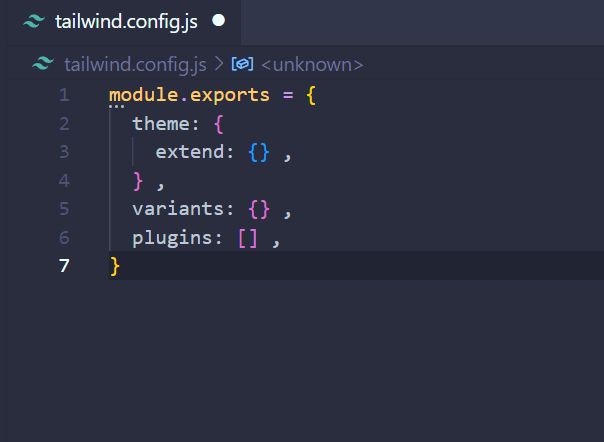
\includegraphics[scale=1.2]{pics/tailwind-config.PNG}
  \caption{\label{fig:Tailwind}Tailwind - config-Datei }
\end{figure}

Sobald man die vorgefertigten CSS-Klassen nutzen will oder bereits selbst 
benutzerdefinierte Klassen selbst hinzugefügt hat, kann man den Erstellungsprozess (build) starten.
\begin{figure}[ht!]
  \centering
  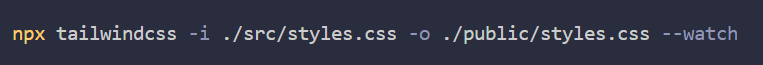
\includegraphics[scale=1]{pics/build-tailwind.PNG}
  \caption{\label{fig:Tailwind}Tailwind - Erstellungsprozess starten }
\end{figure}



\section{React 18.2.0}
React ist eine \textbf{JavaScript-Programmbibliothek} zur Erstellung von webbasierten Benutzeroberflächen. 
Jede React-Webanwendung besteht aus wiederverwendbaren Komponenten, die Teile der Benutzeroberfläche bilden - wir können 
eine separate Komponente für unsere Navigationsleiste haben, eine für die Fußzeile, eine andere für den Hauptinhalt und so weiter. 

Diese wiederverwendbaren Komponenten machen die Entwicklung einfacher, weil man wiederkehrenden Code nicht wiederholen muss. 
Man muss nur die Logik erstellen und die Komponente in jeden Teil des Codes importieren, in dem sie benötigt wird.
React ist außerdem eine Single-Page-Anwendung. Anstatt also jedes Mal, wenn eine neue Seite gerendert werden soll, eine Anfrage 
an den Server zu senden, wird der Inhalt der Seite direkt von den React-Komponenten geladen. Das führt zu einem schnelleren 
Rendering ohne Neuladen der Seite.

In den meisten Fällen wird für die Erstellung von React-Apps die Syntax JSX (JavaScript XML) verwendet, eine Syntaxerweiterung 
von JavaScript. Damit kann man die Logik von JavaScript und die Logik der Benutzeroberfläche auf einzigartige Weise kombinieren. 
Mit JSX muss kein DOM integriert werden, weil man einfach Methoden wie \textbf{document.getElementById}, \textbf{querySelector} 
und andere DOM-Manipulationsmethoden verwendet.
Die Verwendung von JSX ist zwar nicht obligatorisch, aber sie macht die Entwicklung von React-Anwendungen einfacher.

React kann mit Technologien wie Bootstrap, Tailwind CSS, Firebase und vielen mehr, kombiniert werden. 
Außerdem kann React auch mit Node.js und anderen Backend-Sprachen verwendet werden, um Full-Stack-Anwendungen und Web-Apps zu
erstellen. 

\subsection*{Komponenten}
In React ist jedes UI-Element eine Komponente. Es gibt zwei Arten um Komponenten: Klassenkomponenten und Funktionskomponenten. Die neue moderne Variante 
sind Funktionskomponenten, die Hooks als neue Funktion integriert haben. Mehr zu Hooks später.
Komponenten haben einen ähnlichen Aufbau wie Funktionen in Javascript und geben einen HTML-Code mit oft dynamischen Werten zurück.
Der Name der Komponente muss mit einem Großbuchstaben beginnen, denn sonst würde sie nicht funktionieren.

Das Erstellen einer neuen React-Komponente funktioniert folgendermaßen.

\begin{lstlisting}[caption=Komponente in React]
  function LoginButton {
    return (
        <div className="login-container">
          <button className="login-btn">
              Authenticate
          </button>
        </div>
    )
}

export default LoginButton
\end{lstlisting}

In diesem Beispiel wird ein einfacher Button initialisiert. Dieser Button kann dann ganz einfach mit ``<LoginButton />''
als UI-Element in einer anderen Komponente platziert werden. Wichtig für das Verwenden der Komponente ist das Exportieren 
in der letzten Zeile im Beispiel ``export default LoginButton''.

\subsection*{Events}
In React werden Events in CamelCase-Syntax geschrieben werden. Das bedeutet, dass zum Beispiel aus ``onclick'' in 
einem anderen Framework mit ``OnClick'' geschrieben wird. 

Wenn ein Event als Attribut in einem HTML-Tag übergeben wird, dann verwendet man die geschweiften Klammern: onClick{changeName}

\begin{lstlisting}[caption=React Event]
  function LogoutButton() {

    const auth = useAuth();

    const handleClick = () => {
        auth.removeUser().then(r => console.log(r));
    }

    return (
        <button className="logout-btn" onClick={() => handleClick()}>
            Log out
        </button>
    )
}

export default LogoutButton
\end{lstlisting}

Im obigen Beispiel wird die Funktion ``handleClick()'' aufgerufen, sobald auf den Button geklickt wird.


\subsection*{Status / State in React}
In React ist es so, dass in funktioinalen Komponenten, Änderungen an der Statusvariable nicht im DOM angezeigt werden. 
Der Status bleibt unverändert. 
\\
Deshalb verwendet man die useState Hook. Hooks ermöglichen es auf zusätzliche React-Funktionen zuzugrifen, ohne 
dafür eine Klasse zu schreiben. Diese Funktionen können beim Verwalten einer Variable behilflich sein.
\begin{lstlisting}[caption=State von Variablen in React]
  const [name, setName] = useState("David");
  const changeName = () => {
      setName("Daniel");
  };
\end{lstlisting}

Im Beispiel wird eine Statusvariable namens name und eine Funktion - setName - erstellt. Der ursprüngliche Wert der name Variable
``David'' wird in der useState Hook gespeichert. In der Funktion changeName wird dann die Funktion setName verwendet, um den Wert
der name Variable zu ändern.

\subsection*{Hooks}
Es gibt natürlich nicht nur die useState Hook in React, sondern sehr viele Andere auf die hier nicht alle eingegangen werden kann.
Die useEffect Hook ist eine weitere bekannte und oft verwendete Hook.
Der Nutzen kann so erklärt werden, dass jedes Mal ein Effekt ausgeführt wird, wenn sich ein Status ändert.
Stanardmäßig wird diese Hook beim ersten Rendering und bei jeder Aktualisierung des Status ausgeführt. 
Man kann den Effekt jedoch auch an eine entsprechende Statusvariable anhängen.

\begin{lstlisting}[caption=Hook in React]
  function App() {
    const [day, setDay] = useState(1);
    useEffect(() => {
        console.log(`You are in day ${day} of the year`);
    });
    return (
        <div>
        <button onClick={() => setDay(day + 1)}>Click to increase day</button>
        </div>
    );
}
export default App
\end{lstlisting}
Beim Klicken des Buttons, wird die Variable day um eins erhöht. Die Änderung des Wertes führt dazu, dass die useEffect Hook
ausgelöst wird und die Änderung in der Konsole protokolliert. Das geschieht jedes Mal, wenn sich die Variable ändert.

\subsection*{Props}
Um Daten von einer Komponente an eine andere weiterzugeben, werden props verwendet. Das macht den Datenfluss in der App 
dynamisch. Props ist die Abkürzung für Properties, also Eigenschaften.

Zur Demonstration werden zwei Komponenten benötigt, um Daten von der einen zu anderen Komponente zu übertragen.
\begin{lstlisting}[caption=Props in React]
  function User({name, age}) {
    return (
        <div>
        <p>My name is { name }</p>
        <p>I am { age } old</p>
        </div>
    );
}
export default User
\end{lstlisting}

Die User Komponente besitzt in dem Beispiel zwei Parameter (props) deren Wert in einer anderen Komponente bestimmt werden kann.

\begin{lstlisting}[caption=Props Beispiel 2 in React]
  import User from "./User";
  
  function App() {
      return (
          <div className="container">
            <User name="James" age="19"/>
          </div>
      );
  }
  export default App;
\end{lstlisting}\cite{APCW2009}




\clearpage

\section{REST}
REST (Representational State Transfer) wurde entwickelt, um 
bereits existierende Vorteile bestehender Protokolle zu nutzen. 
Die Programmierschnittstelle beschreibt einen Ansatz für die 
Kommunikation zwischen Client und Server in Netzwerken, zum Austausch von Informationen und Daten. 
Die Daten werden in einer RESTful API in verschiedenen Notationssprachen übermittelt, wobei 
JSON (JavaScript Object Notation) und XML (Extensible Markup Language) die beiden häufigsten Format sind.
Beide Formate sind textbasiert und können vom Menschen leicht gelesen werden.
\begin{figure}[ht!]
  \centering
  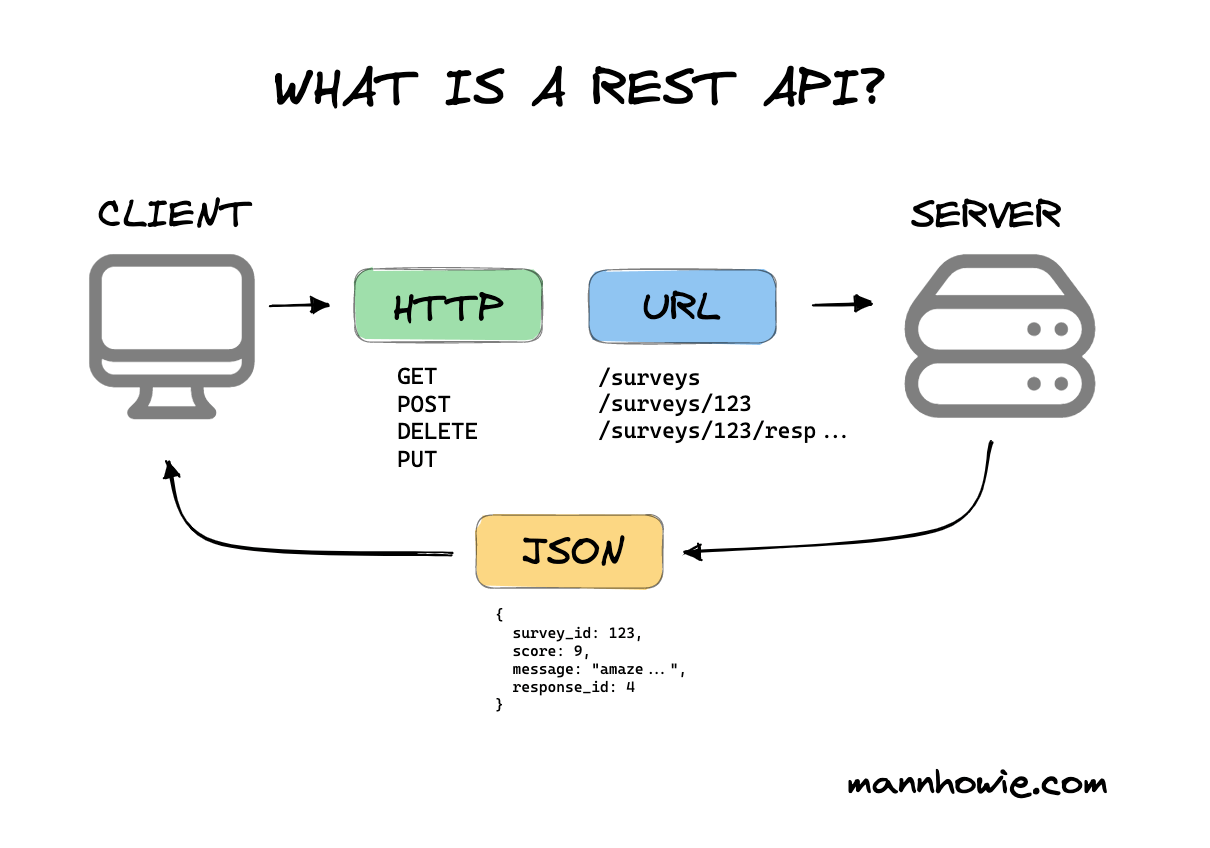
\includegraphics[scale=.4]{pics/rest-api.png}
  \caption{\label{fig:The-caption}REST-API \cite{APCW20011}}
  \label{fig:impl:use-case-diagramm}
\end{figure}
\\
REST stellt eine Alternative zu anderen Schnittstellen wie SOAP oder WSDL dar, ist
dabei aber weder Protokol noch Standard. Die Architektur bedient sich dabei 
an standardisierte Verfahren wie HTTP, JSON oder XML.
\\
In der Praxis wird Rest bevorzugt mit HTTP(S) realisiert. Die Services 
werden per URL/URI angesprochen. Die HTTP-Methoden geben an welche Operation
von dem Dienst ausgeführt werden soll.\cite{APCW20010}
\\
\subsection{HTTP-Methoden}
Das World Wide Web liefert bereits die nötige Infrastruktur für die 
REST-Schnittstelle, deswegen kann es auch sofort mit einem Browser
ausprobiert werden. Zur Hilfe kommen dabei sogennante Fake Online APIs 
die das Testen der Schnittsetellen vereinfachen. 
Für das Arbeiten mit RESTful APIs gibt es vier HTTP-Methoden.

\begin{itemize}
  \item {\textbf{GET} fordert Daten vom Server an, zum Beispiel alle Benutzer mit dem Namen ``John''.}
  \item {\textbf{POST} schickt Daten an den Server, zum Beispiel wenn ein neuer Nutzer angelegt wird. }
  \item {\textbf{PUT} aktualisiert beziehungsweise ändert bestehende Datensätze auf dem Server. Ein Beispiel dafür wäre,
  wenn der Name eines Users von ``John'' auf ``Joe'' geändert werden soll. }
  \item {\textbf{DELETE} löscht Daten auf dem Server, zum Beispiel ein inaktiver Benutzer soll entfernt werden. }
\end{itemize}\cite{APCW20012}

\subsection{JSON}

\subsection*{Allgemein}
JSON (JavaScript Object Notation) ist ein unabhängiges Datenformat und mit der sehr einfachen menschenlesbaren Struktur, das ideale Format, um Daten
zwischen Systemen auszutauschen. Es wird im Unicode Zeichensatz kodiert und wird zwischen Anwendungen immer als Ganzes 
ausgetauscht. Der Inhalt eines JSON Dokuments ist Objektorientiert aufgebaut und die Datei endet mit ``.json''.
\\
Die Formatierung eines JSON-Dokuments muss eine genau Struktur haben. Es wird mit \{ begonnen und mit \} beendet. Zwischen den 
Klammern befinden sich die Inhalte. Die geschweiften Klammern umfassen ein Objekt. Es gibt auch Verschachtelungen in denen im Objekt
weitere Objekte definiert werden können. JSON funktioniert mit Key-Value Paaren, das heißt, dass ein Datenfeld immer mit einem 
Namen eingeleitet wird und nach dem Doppelpunkt folgt ein Wert. \cite{APCW20013}
\\
\subsection*{Datentypen}
Zeichenketten, sind beliebige Texte der zwischen Anführungszeichen platziert wird. Diese Zeichenkette wird auch String 
genannt. 
\begin{lstlisting}[caption=JSON Datentyp String]
  {
    "name": "John Doe",
  }
\end{lstlisting}

Boolean ist ein Wahrheitswert und kann entweder true oder false annehmen. Der Wert wird ohne Anführungszeichen geschrieben.
\begin{lstlisting}[caption=JSON Datentyp Boolean]
  {
    "name": "John Doe",
    "isStudent": true,
  }
\end{lstlisting}

Eine Zahl wird mit den Ziffern 0-9 und optional mit einem Punkt und Vorzeichen dargestellt. Auch ein Exponent kann 
genutzt werden. 
\begin{lstlisting}[caption=JSON Datentyp Number]
  {
    "name": "John Doe",
    "isStudent": true,
    "age": 25
  }
\end{lstlisting}

Das sind die wichtigsten drei Typen, es gibt natürlich noch viele weitere Möglichkeiten Daten in JSON-Dokumenten darzustellen, wie
Objekte, Arrays und mehr. Wenn man ausdrücken will, dass eine Variable leer ist, kann man das mit ``null'' ausdrücken. 
\cite{APCW20014}
\\
\\
Im Projekt hat die JSON Notation eine Rolle gespielt, weil die Daten die von der API zum Anzeigen ins Frontend geholt wurden 
im JSON-Format waren, was üblich für den Datenaustausch zwischen API und Anwendung ist.


\subsection{HTTP Status Codes}
Mithilfe von Status Codes, teilt eine REST-API dem Benutzer, das Resultat der Anfrage mit.
Die Server Antwort besteht aus einer dreistelligen Zahl und einer kurzen
Beschreibung.
\\
Es gibt fünf verschiedene Statusklassen. Die erste Ziffer der steht dabei immer 
für die jeweilige Klasse.

\begin{itemize}
  \item {\textbf{Informative Antworten (100-199)} wie zum Beispiel ``102 - In Bearbeitung''. }
  \item {\textbf{Erfolgreiche Antworten(200-299)} wie ``200 - OK''. }
  \item {\textbf{Umleitungen(300-399)} auf eine andere Adresse. Das Dokument ist auf einer anderen Adresse
  erreichbar. }
  \item {\textbf{Client-Fehler(400-499)} , also eine fehlerhafte Anfrage auf Client-Seite wie zum Beispiel
  ``404 - nicht gefunden''. }
  \item {\textbf{Server-Fehler(500-599)} sind Fehler die auf den Server zurückgehen, wie 
  zum Beispiel ``500 - Interner Server-Fehler''. }
\end{itemize} \cite{APCW20015}



